\documentclass{article}
\usepackage{graphicx} % Required for inserting images
\usepackage{amsmath}      % For advanced math formatting
\usepackage{amssymb}      % For mathematical symbols
\usepackage{mathtools}    % Enhanced math formatting
\usepackage{geometry}     % For page margins
\usepackage{hyperref}     % For clickable references
\usepackage{booktabs}     % For professional tables
\usepackage{natbib}       % For citations
\usepackage[font=small]{caption}

% Page setup
\geometry{
    a4paper,
    margin=2.5cm
}

\title{Traffic Congestion Analysis}
\author{Alexandre Crivellari - 902064}
\date{January 2025}

\begin{document}

\maketitle

\section{Introduction}

\subsection{Project Overview and Objectives}
Traffic congestion prediction represents a critical component in modern urban traffic management systems. This study focuses on developing and comparing multiple forecasting approaches for predicting traffic congestion levels on a major U.S. freeway. The primary objective is to generate accurate hourly predictions using a combination of statistical and machine learning methods, providing insights into traffic patterns and their underlying determinants.

Our analysis employs three distinct modeling approaches: a Seasonal Autoregressive Integrated Moving Average model with exogenous variables (SARIMAX), an Unobserved Components Model (UCM), and an XGBoost-based machine learning model. Each approach offers unique advantages in capturing different aspects of the time series dynamics, from explicit seasonal patterns to complex non-linear relationships.

\subsection{Description of the Traffic Congestion Dataset}
The dataset comprises hourly traffic congestion measurements spanning from January 2015 through November 2016, recorded as a continuous time series. The congestion indicator, denoted as $X_t$, represents a normalized measure of traffic density, where higher values indicate increased congestion levels. Each observation is timestamped with both date and hour components, allowing for detailed temporal pattern analysis.

\subsection{Forecasting Challenge: One Month of Hourly Predictions}
The core challenge of this project involves generating 744 consecutive hourly forecasts, representing a complete month of traffic congestion predictions. This extended forecast horizon presents several technical challenges:

\begin{enumerate}
    \item Long-range dependency modeling: Traffic patterns exhibit both daily (24-hour) and weekly seasonality
    \item Accumulated uncertainty: Forecast uncertainty naturally grows with the prediction horizon
    \item Special period handling: The forecast period may include holidays or other special events that could affect traffic patterns
\end{enumerate}

\subsection{Overview of Selected Modeling Approaches}
Our methodology employs three complementary approaches:

1. SARIMAX Modeling: We implement a SARIMAX(2,1,2)(1,1,1)$_{24}$ model with weekly pattern exogenous variables:
   \begin{equation}
   (1-\phi_1B-\phi_2B^2)(1-\Phi_1B^{24})(1-B)(1-B^{24})X_t = (1+\theta_1B+\theta_2B^2)(1+\Theta_1B^{24})\varepsilon_t + \beta W_t
   \end{equation}
   where $B$ is the backshift operator, $W_t$ represents the weekly seasonal pattern through a phase-adjusted sine component.

2. Unobserved Components Model (UCM): This approach decomposes the series with a local level and stochastic daily seasonality:
   \begin{equation}
   X_t = \mu_t + \gamma_t + \beta W_t + \varepsilon_t, \quad \mu_t = \mu_{t-1} + \eta_t
   \end{equation}
   where $\mu_t$ is the local level component, $\gamma_t$ represents the 24-hour stochastic seasonal component, and $W_t$ captures the weekly pattern through exogenous variables.

3. XGBoost Model: We employ an extreme gradient boosting framework with specific lag features:
   \begin{equation}
   \hat{X}_t = f(X_{t-1}, X_{t-24}, W_t) = \sum_{k=1}^K f_k(X_{t-1}, X_{t-24}, W_t)
   \end{equation}
   where $f_k$ represents individual tree predictors trained on one-hour and 24-hour lags, along with the weekly pattern features $W_t$.

Each approach leverages different aspects of the time series structure: SARIMAX captures linear dependencies and explicit seasonality, UCM handles evolving patterns through its state-space formulation, and XGBoost captures complex non-linear relationships through its tree-based architecture.

\section{Data Understanding and Preprocessing}

\subsection{Dataset Structure and Components}
The traffic congestion data is structured as a regular time series with hourly granularity, spanning from January 2015 through November 2016. The dataset comprises four primary fields:

\begin{itemize}
\item \texttt{DateTime}: A timestamp field combining both date and hour information, serving as the primary temporal index
\item \texttt{Date}: The calendar date component in YYYY-MM-DD format
\item \texttt{Hour}: An integer field (0-23) representing the hour of day
\item \texttt{X}: The target variable representing traffic congestion levels
\end{itemize}

The time series exhibits several structural characteristics that influence our modeling approach:

\begin{itemize}
\item \textbf{Temporal Resolution}: Hourly measurements provide sufficient granularity to capture both intra-day variations and longer-term patterns
\item \textbf{Regular Spacing}: Observations are consistently spaced at one-hour intervals, simplifying the application of traditional time series methods
\item \textbf{Multiple Seasonality}: The data structure inherently supports analysis of:
  \begin{itemize}
  \item Daily patterns (24-hour cycle)
  \item Weekly patterns (168-hour cycle)
  \item Monthly variations (approximately 720-hour cycle)
  \end{itemize}
\end{itemize}

The target variable X represents a normalized measure of traffic congestion, with several key properties:
\begin{itemize}
\item \textbf{Range}: Values are non-negative, reflecting physical constraints of traffic measurement
\item \textbf{Scale}: The measurements appear to be normalized, facilitating direct comparison across different time periods
\item \textbf{Resolution}: Sufficient numerical precision to capture subtle variations in congestion levels
\end{itemize}

This structured format enables the application of various time series analysis techniques while maintaining the interpretability of the results. The combination of both date and hour components allows for flexible aggregation and pattern analysis at multiple temporal scales, which proves crucial for our multi-model forecasting approach.

\subsection{Data Quality Assessment}
A comprehensive assessment of data quality revealed several characteristics requiring attention for robust time series analysis. The evaluation focused on three key aspects: missing value patterns, edge cases, and data integrity.

\subsubsection{Missing Values Analysis}
The time series data exhibits specific patterns of missing values that required systematic treatment:
\begin{itemize}
    \item \textbf{Daylight Saving Time Gaps}: Two specific timestamps were identified as missing:
    \begin{itemize}
        \item March 29, 2015, 02:00:00
        \item March 27, 2016, 02:00:00
    \end{itemize}
    These gaps correspond to daylight saving time transitions and were addressed through localized interpolation using adjacent day values.
\end{itemize}

\subsubsection{Treatment of Edge Cases}
Several edge cases were identified and treated:
\begin{enumerate}
    \item \textbf{Duplicate Timestamps}: A small number of duplicate timestamps were detected in the dataset. These were resolved by:
    \begin{itemize}
        \item Computing the mean value for X at identical timestamps
        \item Retaining the first occurrence of date and hour information
        \item Ensuring chronological ordering after deduplication
    \end{itemize}
    
    \item \textbf{Outlier Analysis}: Using the Interquartile Range (IQR) method:
    \begin{equation}
        \text{Outlier if } X < (Q_1 - 1.5 \times \text{IQR}) \text{ or } X > (Q_3 + 1.5 \times \text{IQR})
    \end{equation}
    where $Q_1$ and $Q_3$ represent the first and third quartiles respectively.
\end{enumerate}

\subsubsection{Data Integrity Checks}
Several validation procedures were implemented to ensure data integrity:

\begin{enumerate}
    \item \textbf{Time Series Continuity}: A verification process confirmed that observations where consistently hourly spaced and in the proper chronological order.
    
    \item \textbf{Value Distribution Analysis}: Values for the traffic congestion indicator where confirmed non-negative and not-outliers.
\end{enumerate}

Following these quality assessments, appropriate cleaning procedures were implemented to ensure data reliability while preserving the inherent characteristics of the traffic patterns. The cleaned dataset maintains the temporal integrity necessary for accurate time series modeling while addressing potential sources of bias or error in the original data.

\section{Exploratory Data Analysis}

\subsection{Temporal Pattern Analysis}
Analysis of the traffic congestion time series reveals complex temporal dynamics operating at multiple scales. Examination of the complete time series spanning from January 2015 to November 2016 shows a remarkably consistent pattern of daily fluctuations, with congestion values typically ranging between 0 and 0.4. This stability in the overall pattern suggests strong seasonal components that persist across years.

\begin{figure}[htbp]
    \centering
    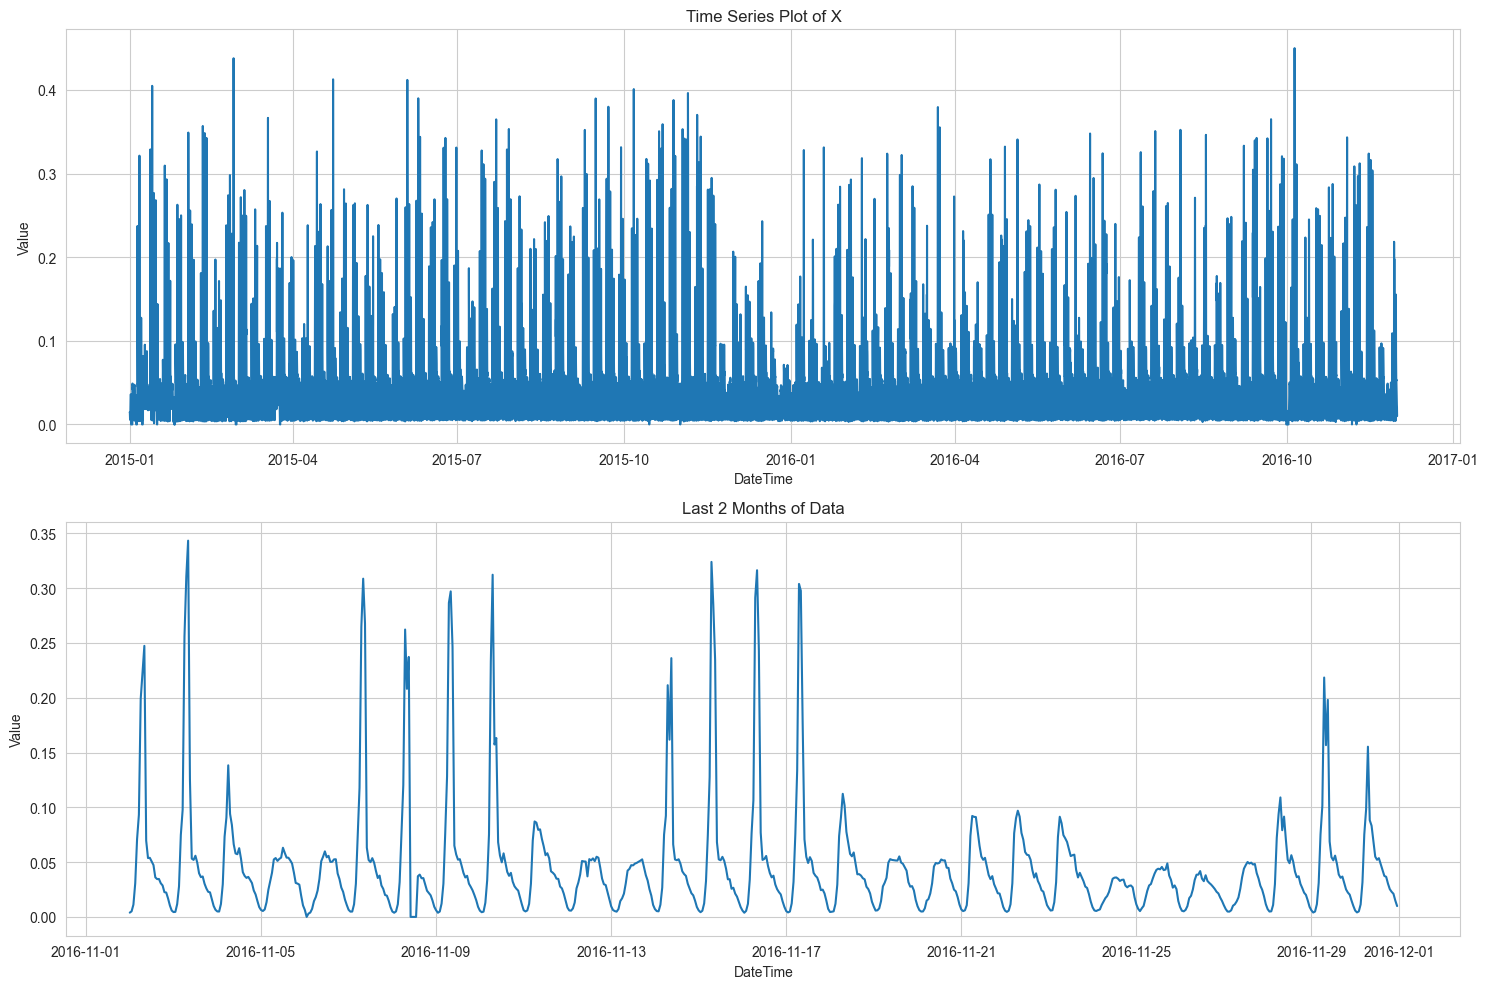
\includegraphics[width=\textwidth]{time_series_full.png}
    \caption{Time series plot of traffic congestion (full period and last two months). The upper panel shows the complete time series from 2015 to 2016, while the lower panel provides a detailed view of the final two months, highlighting the daily pattern structure.}
    \label{fig:time_series}
\end{figure}

A closer examination of the daily traffic patterns reveals a pronounced circadian rhythm in congestion levels. The average daily pattern exhibits a sharp morning peak between 07:00 and 08:00, reaching maximum congestion values around 0.12. This morning surge is followed by a gradual decline throughout the afternoon hours, with congestion levels stabilizing at moderate values before decreasing to their lowest points during the nighttime hours (00:00-04:00).

\begin{figure}[htbp]
    \centering
    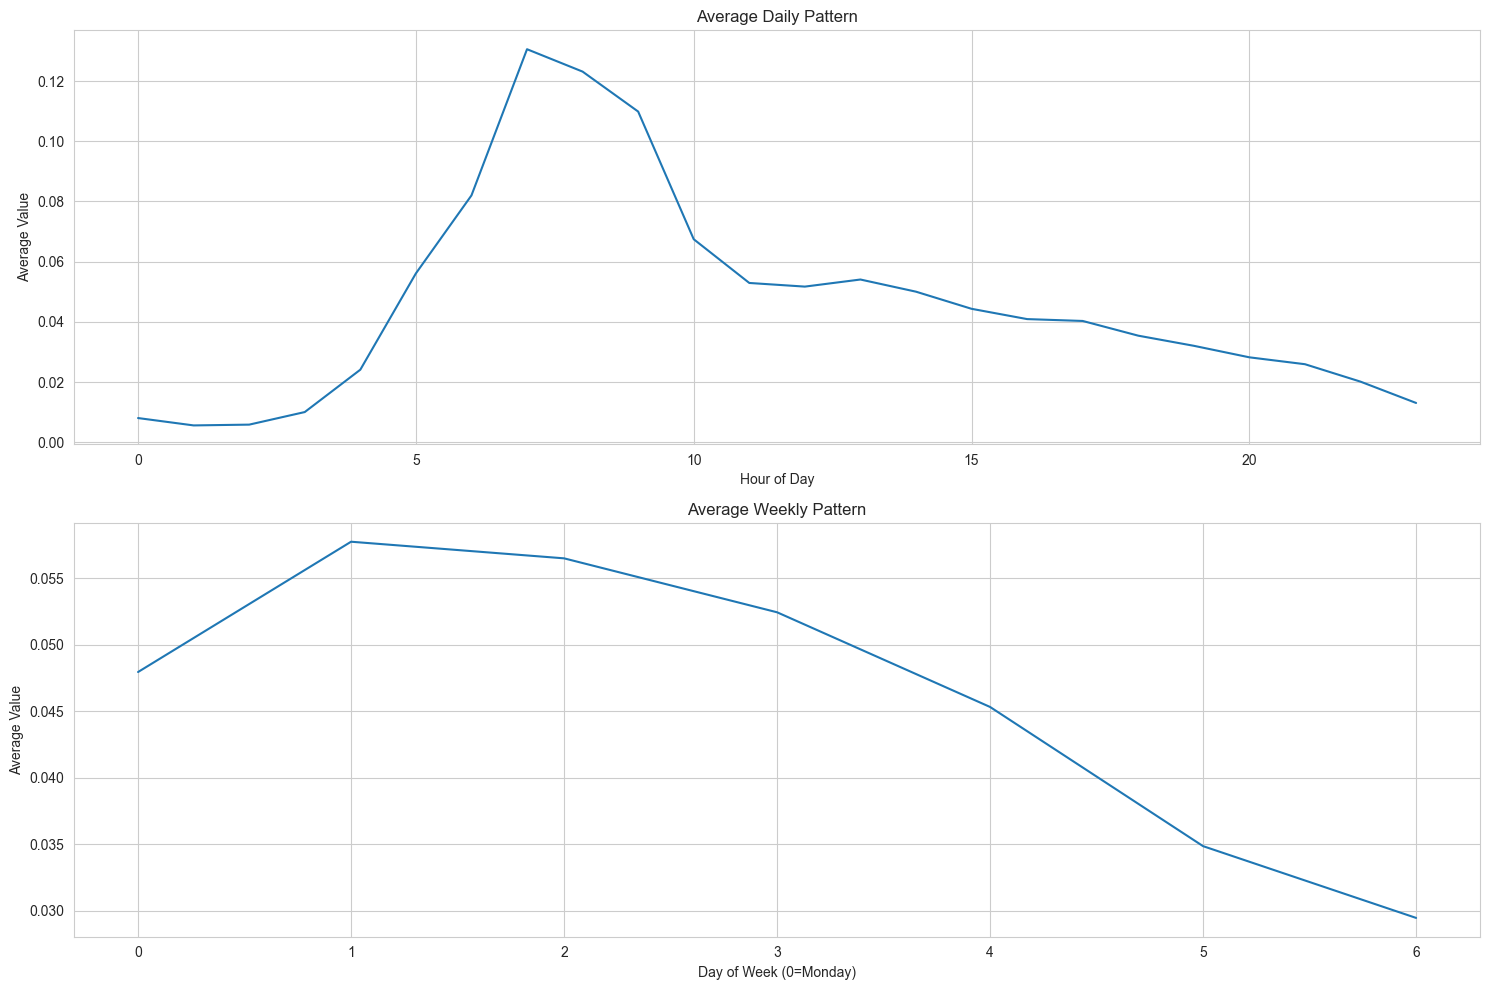
\includegraphics[width=\textwidth]{daily_weekly_patterns.png}
    \caption{Average daily and weekly patterns in traffic congestion. The upper panel shows the 24-hour cycle with its characteristic morning peak, while the lower panel illustrates the weekly variation from Monday (0) to Sunday (6).}
    \label{fig:patterns}
\end{figure}

The weekly cycle presents another significant temporal pattern in the data. Traffic congestion tends to peak during the midweek period, specifically on Tuesdays and Wednesdays, with average values around 0.057. From this peak, congestion levels gradually decrease towards the weekend, reaching their lowest points on Sundays with values around 0.03. This pattern clearly reflects the influence of workplace commuting on traffic patterns, with reduced congestion during weekends when fewer people travel for work.

These systematic patterns in both daily and weekly cycles suggest the need for a modeling approach that can effectively capture multiple seasonal components. The consistency of these patterns also indicates that while the time series exhibits clear seasonality at both daily and weekly scales, the underlying process generating these patterns remains relatively stable over the observed period.

\subsection{Statistical Properties}
Decomposition of the time series into its constituent components reveals the underlying structure of the traffic congestion patterns. A seasonal decomposition using a 24-hour period was performed to separate the series into trend, seasonal, and residual components.

\begin{figure}[htbp]
    \centering
    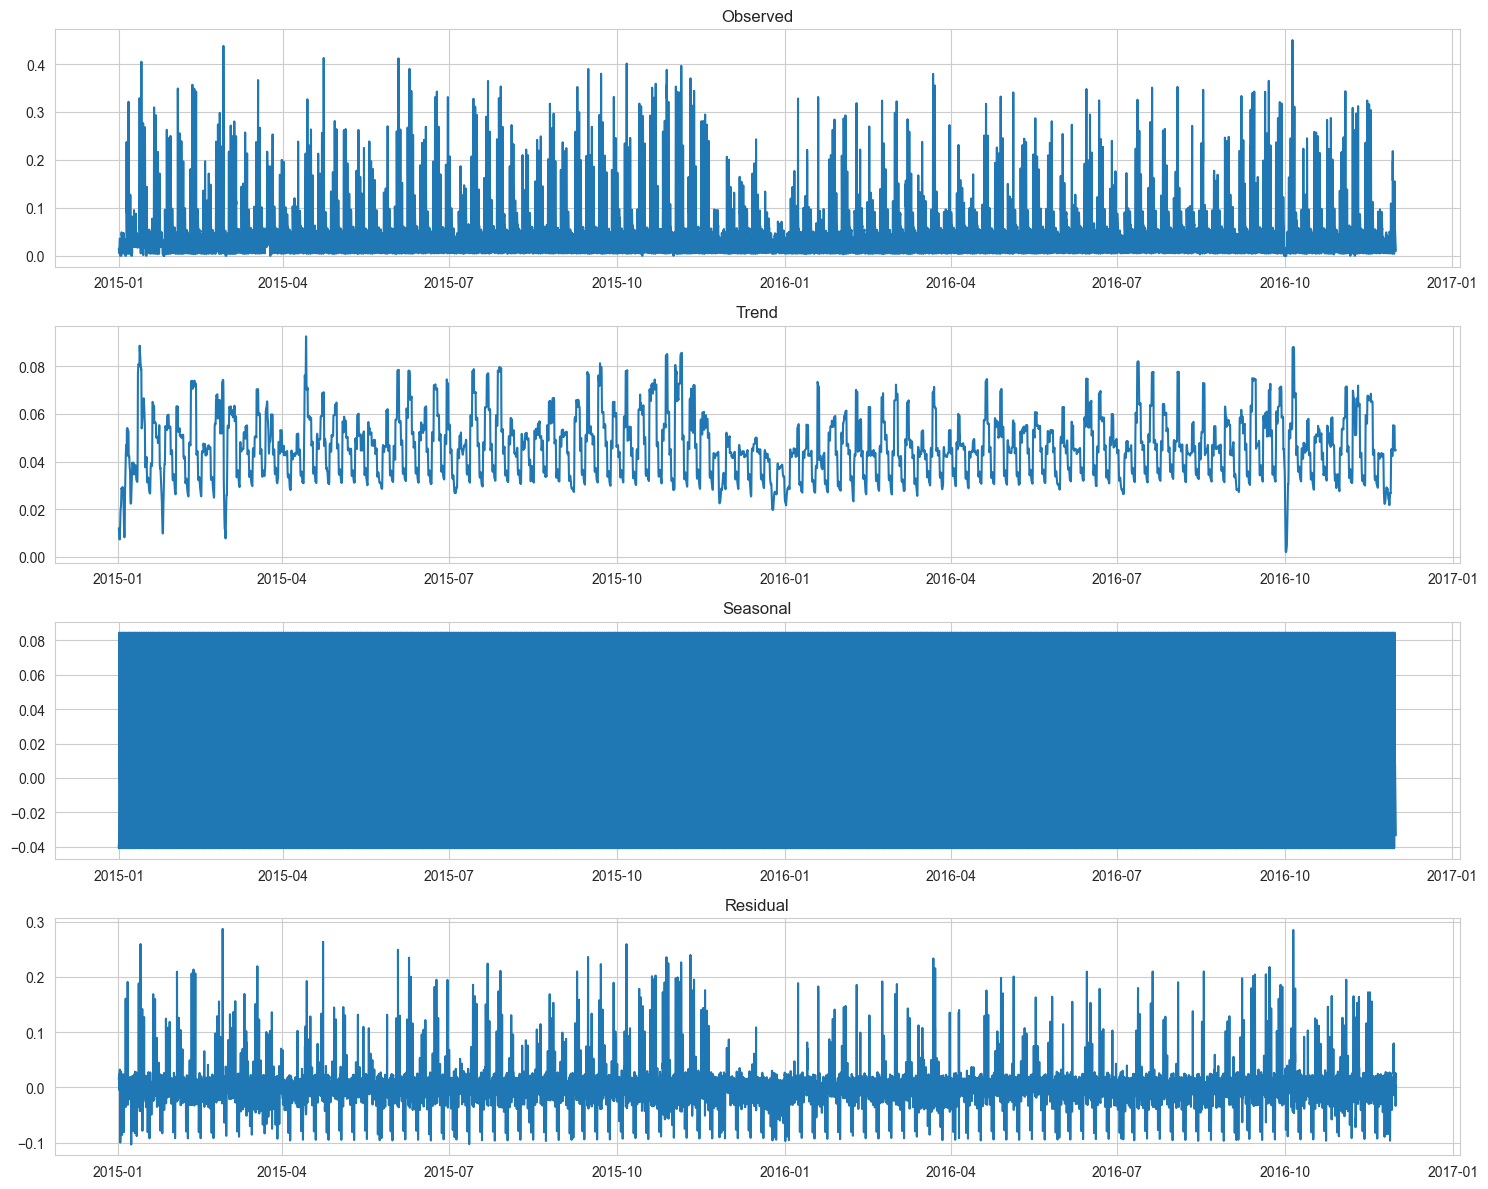
\includegraphics[width=\textwidth]{seasonal_decomp.png}
    \caption{Seasonal decomposition of the traffic congestion time series showing the observed data, trend component, seasonal pattern, and residuals.}
    \label{fig:decomposition}
\end{figure}

The trend component exhibits moderate fluctuations around a relatively stable mean, suggesting no strong long-term directional movement in congestion levels. This stability in the trend indicates that while daily and weekly patterns are prominent, the overall congestion level has remained consistent throughout the observation period.

The seasonal component displays a remarkably regular pattern, capturing the daily cycle of traffic congestion. This regularity reinforces our earlier observations about the strong daily patterns and suggests that the 24-hour seasonality is a fundamental characteristic of the series that should be explicitly incorporated in our modeling approach.

To formally assess the stationarity of the series, we conducted an Augmented Dickey-Fuller (ADF) test. The test yielded a test statistic of -15.71, substantially more negative than the critical values (-3.431, -2.862, and -2.567 at the 1\%, 5\%, and 10\% significance levels, respectively). The corresponding p-value of 1.37×10$^{-28}$ provides overwhelming evidence against the presence of a unit root, indicating that the series is stationary after accounting for its seasonal components.

The residual component, obtained after removing both trend and seasonal effects, exhibits several notable characteristics:
\begin{itemize}
    \item Relatively constant variance across the observation period, suggesting homoscedasticity
    \item No obvious patterns or systematic behavior, indicating successful removal of seasonal components
    \item Occasional spikes that likely correspond to unusual traffic events or anomalies
\end{itemize}

These statistical properties have important implications for our modeling strategy. The strong stationarity evidence supports the use of standard time series models, while the clear seasonal structure suggests the need for explicit seasonal components. The well-behaved residuals indicate that, after accounting for trend and seasonality, the remaining variations can be effectively modeled using standard error structures.

\subsubsection{Autocorrelation Analysis}
To further understand the temporal dependencies in the series of traffic congestion, we performed a comprehensive correlation analysis using both the autocorrelation function (ACF) and the partial autocorrelation function (PACF) on the original series and various transformations.

\begin{figure}[htbp]
    \centering
    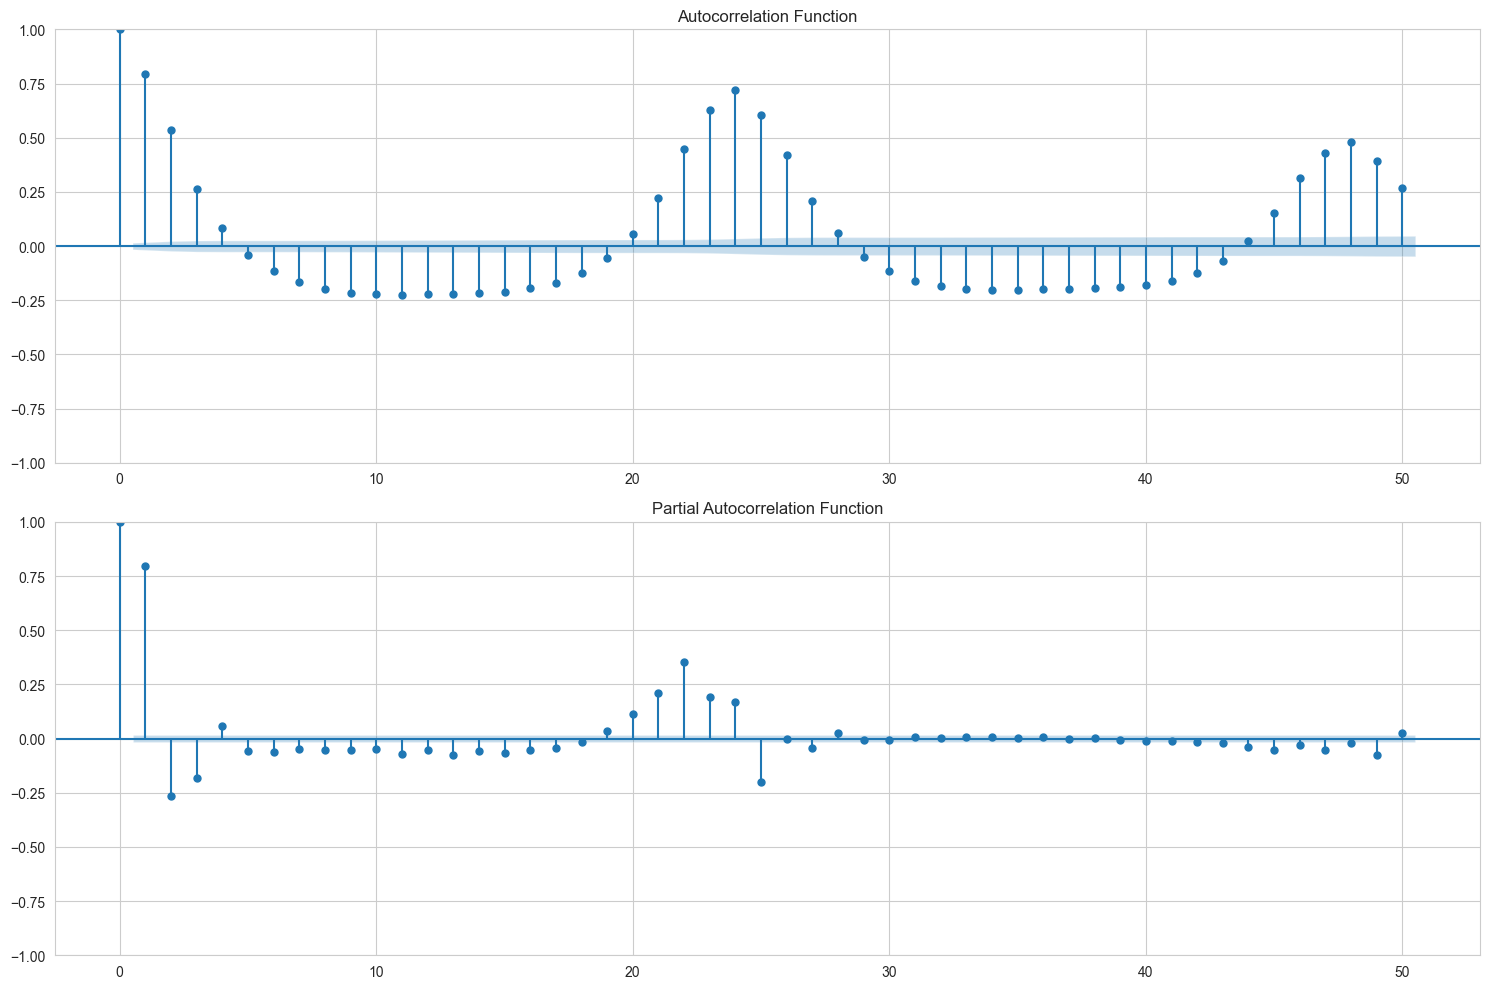
\includegraphics[width=\textwidth]{acf_pacf_original}
    \caption{ACF and PACF of the original series, showing strong periodic correlations at daily (24-hour) intervals.}
    \label{fig:acf_original}
\end{figure}

The ACF of the original series exhibits a distinctive pattern with peaks at regular 24-hour intervals, confirming the strong daily seasonality identified in our decomposition analysis. The slow decay in these peaks suggests the need for seasonal differencing. The PACF shows significant spikes at the first few lags, indicating potential AR(2) behavior in the short-term dynamics.

\begin{figure}[htbp]
    \centering
    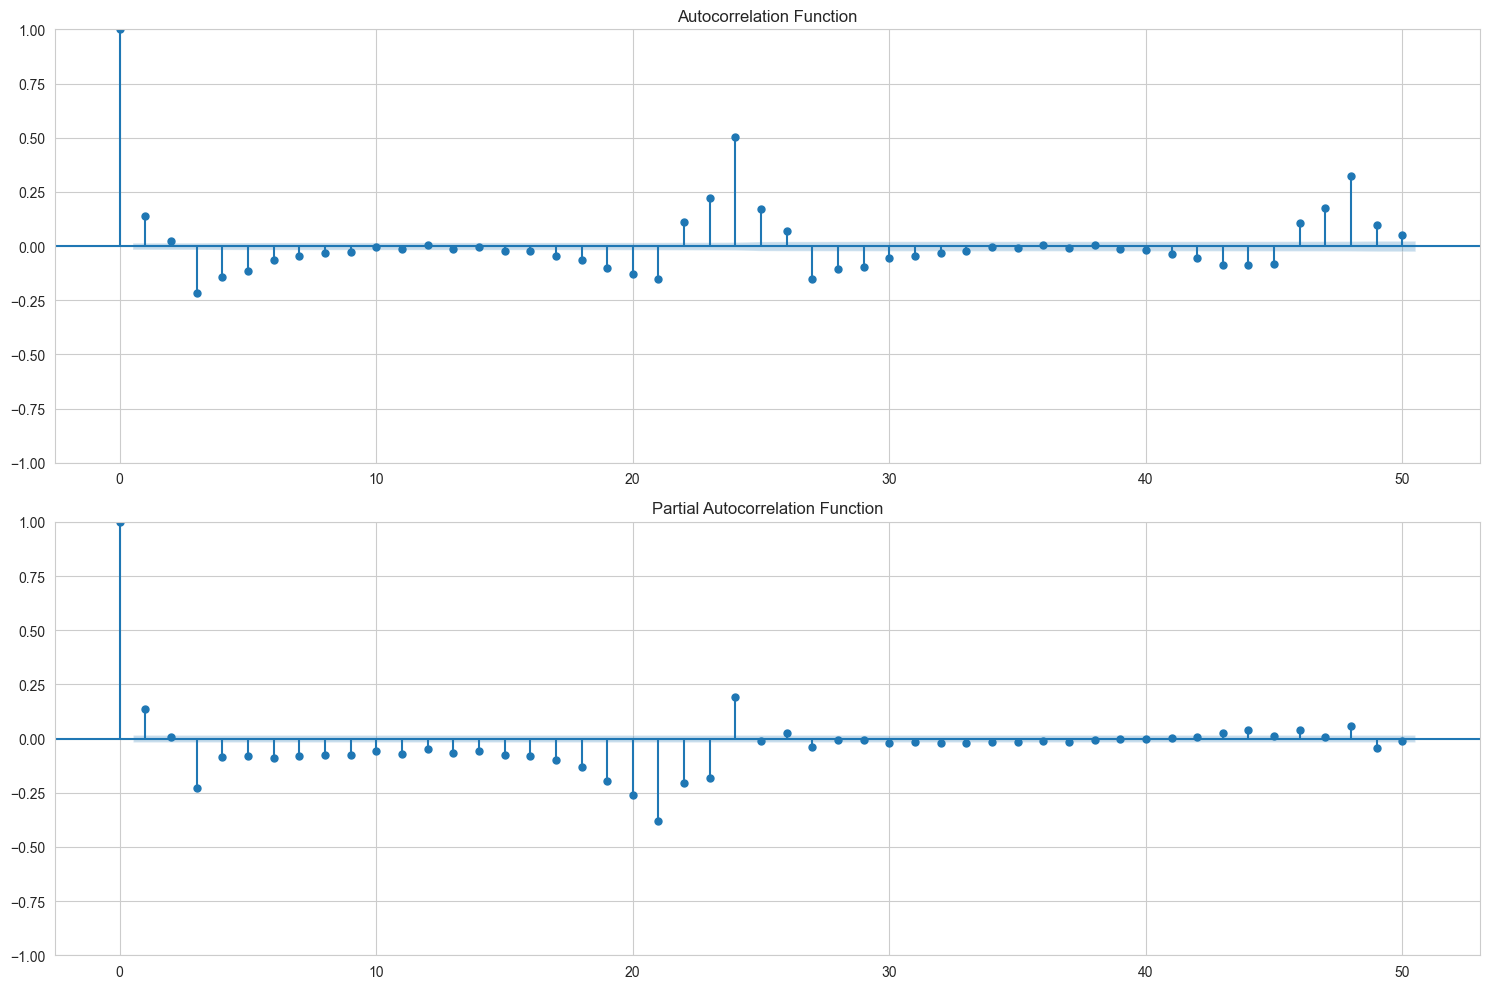
\includegraphics[width=\textwidth]{acf_pacf_diff1}
    \caption{ACF and PACF after first-order differencing, revealing the persistence of seasonal patterns.}
    \label{fig:acf_diff1}
\end{figure}

After applying first-order differencing, the ACF and PACF plots reveal that while the overall correlation structure is reduced, significant seasonal correlations persist. This suggests that while regular differencing helps address some of the non-stationarity, it alone is insufficient to capture the series' full dynamics.

\begin{figure}[htbp]
    \centering
    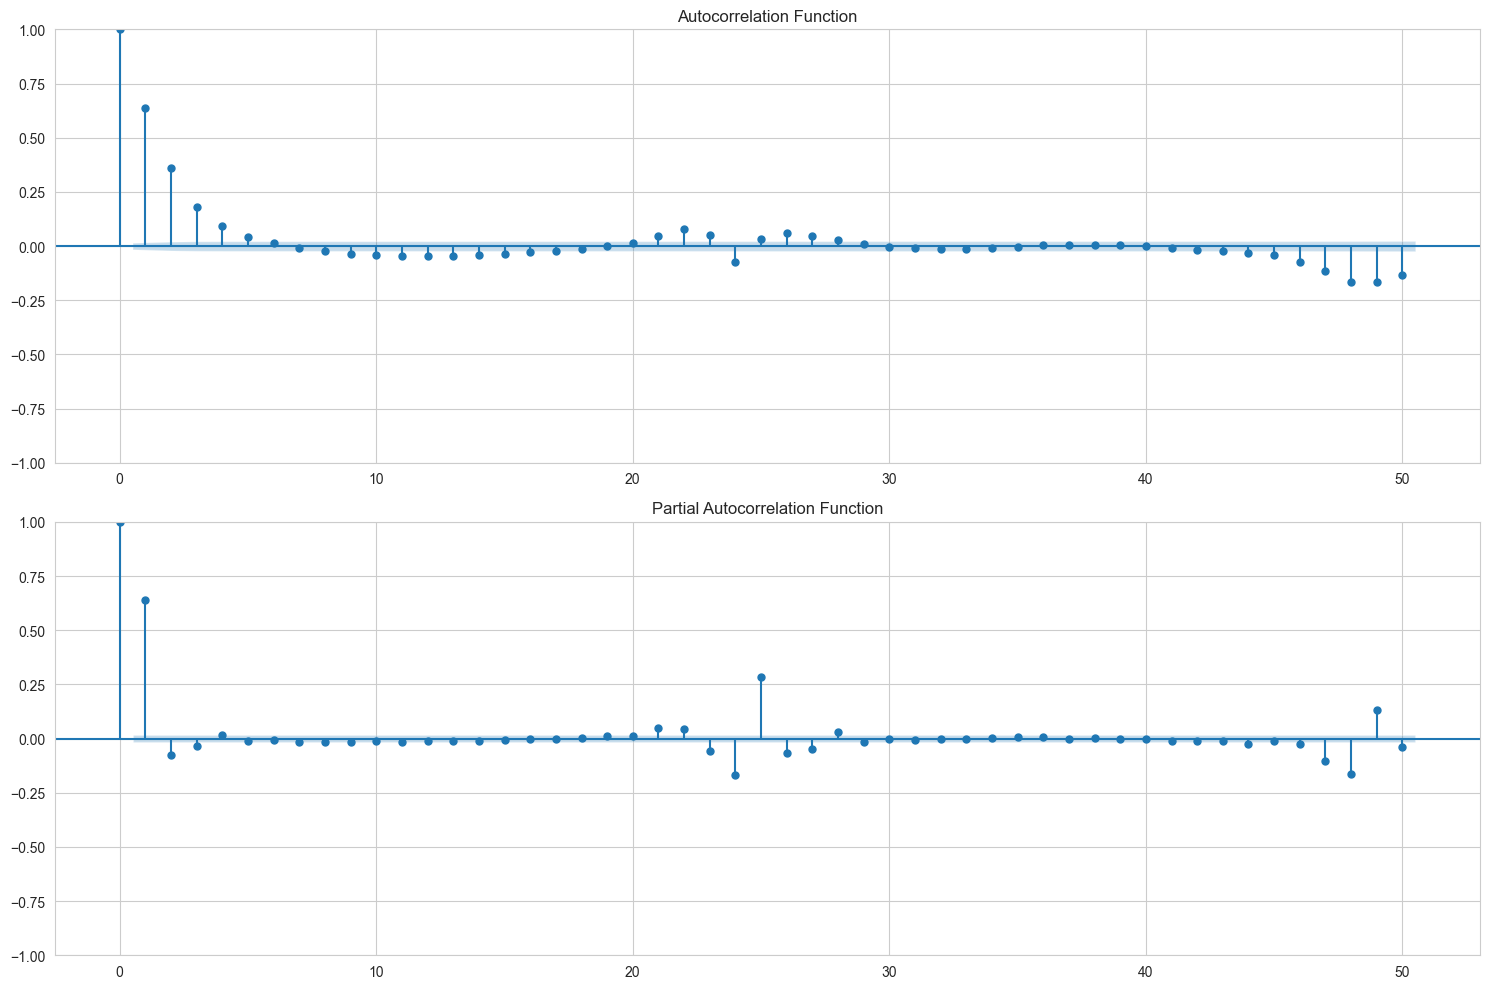
\includegraphics[width=\textwidth]{acf_pacf_seasonal}
    \caption{ACF and PACF of the seasonally differenced series (24-hour period), showing reduced seasonal dependencies.}
    \label{fig:acf_seasonal}
\end{figure}

The seasonally differenced series (lag-24) shows a marked reduction in the periodic correlation structure. The ACF exhibits a more rapid decay, while the PACF suggests the presence of both regular and seasonal autoregressive components. This transformation effectively addresses the strong daily seasonality observed in the original series.

\begin{figure}[htbp]
    \centering
    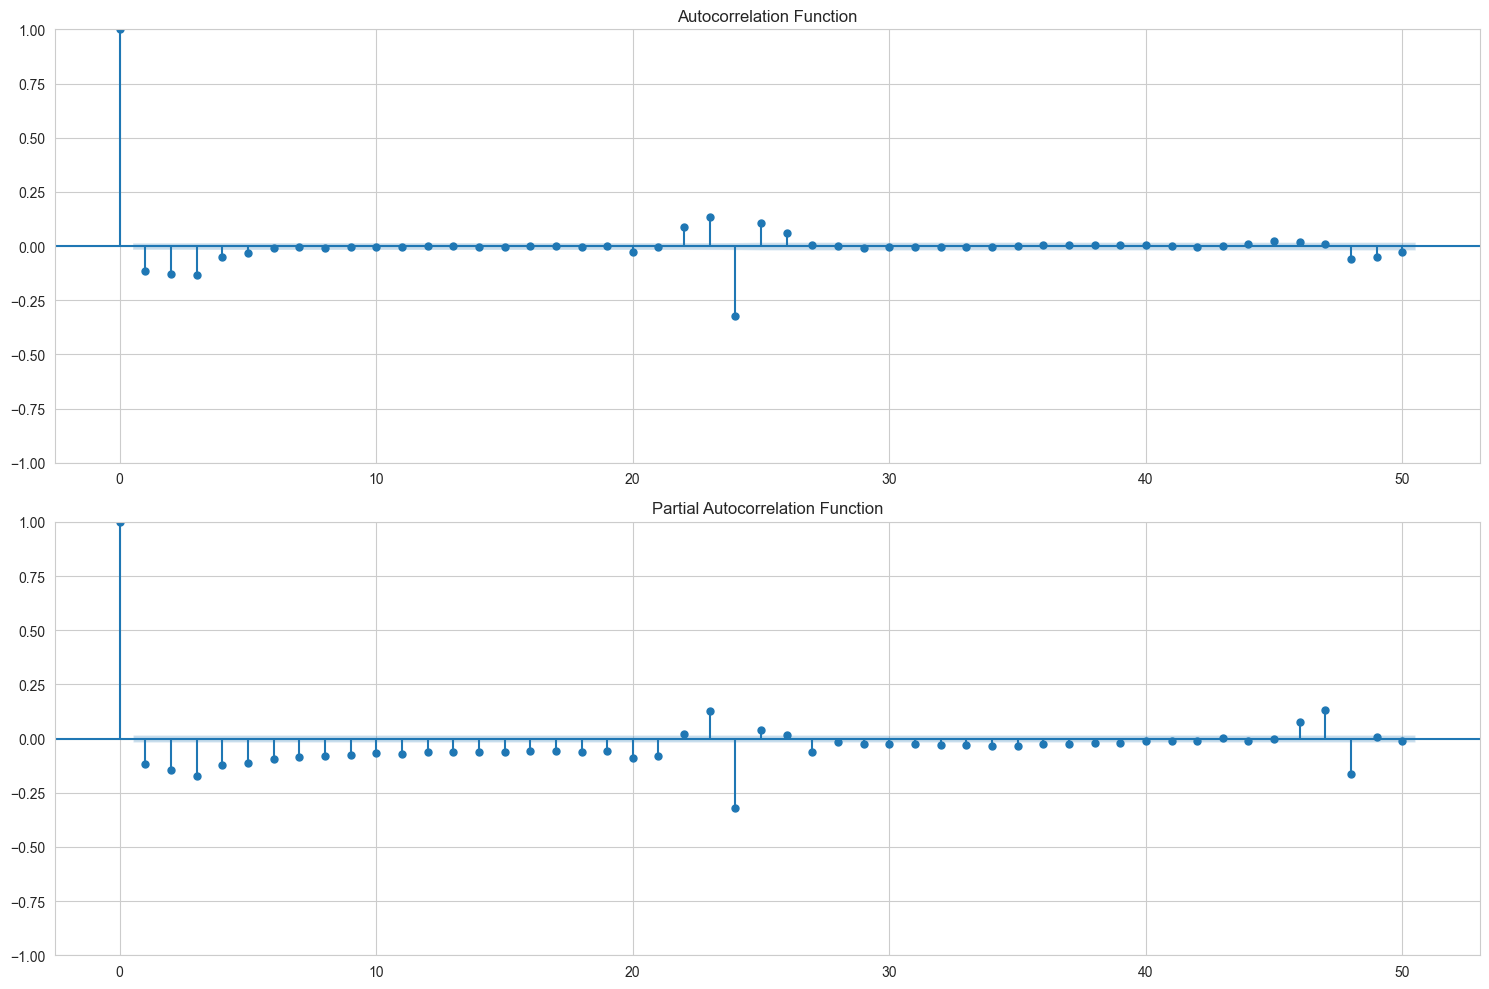
\includegraphics[width=\textwidth]{acf_pacf_both}
    \caption{ACF and PACF after both regular and seasonal differencing, displaying minimal residual correlation structure.}
    \label{fig:acf_both}
\end{figure}

Applying both regular and seasonal differencing produces the most stationary series, with minimal residual correlation structure. The resulting ACF and PACF patterns suggest that a SARIMA model with orders (2,1,2) for the regular component and (1,1,1)$_{24}$ for the seasonal component would be appropriate, as these orders capture the remaining short-term and seasonal dynamics while maintaining model parsimony.

\subsubsection{SARIMA Order Selection}
The determination of SARIMA(2,1,2)(1,1,1)$_{24}$ orders follows from a systematic analysis of both regular and seasonal components in the correlation structure. While the ADF test indicates the series is stationary (test statistic -15.71, p-value 1.37×10$^{-28}$), the strong seasonal patterns in the data suggest that differencing can still improve model performance by simplifying the correlation structure.

\textbf{Regular Component (2,1,2):}
\begin{itemize}
    \item Despite statistical stationarity, we choose differencing order $d=1$ to reduce the complexity of the autocorrelation structure and simplify the model specification.
    \item The AR order $p=2$ is determined from the PACF of the differenced series, which shows significant spikes at lags 1 and 2, followed by a sharp cut-off.
    \item The MA order $q=2$ is selected based on the ACF showing significant correlations at the first two lags, suggesting a second-order moving average process is needed to capture the short-term correlation structure.
\end{itemize}

\textbf{Seasonal Component (1,1,1)$_{24}$:}
\begin{itemize}
    \item The seasonal differencing order $D=1$ is chosen to address the strong periodic correlations at multiples of 24 hours, making the seasonal pattern more manageable.
    \item The seasonal AR order $P=1$ is determined from the PACF at seasonal lags, which shows a significant spike at lag 24 followed by a decay.
    \item The seasonal MA order $Q=1$ is selected based on the ACF at seasonal lags, which exhibits a similar pattern requiring one seasonal moving average term.
\end{itemize}

This specification achieves a balance between model complexity and goodness of fit. While the series is technically stationary, the chosen differencing orders help simplify the underlying patterns, allowing the ARMA components to more effectively capture both the short-term dynamics and daily seasonality.

\subsection{Extended Pattern Analysis}
\begin{figure}[htbp]
    \centering
    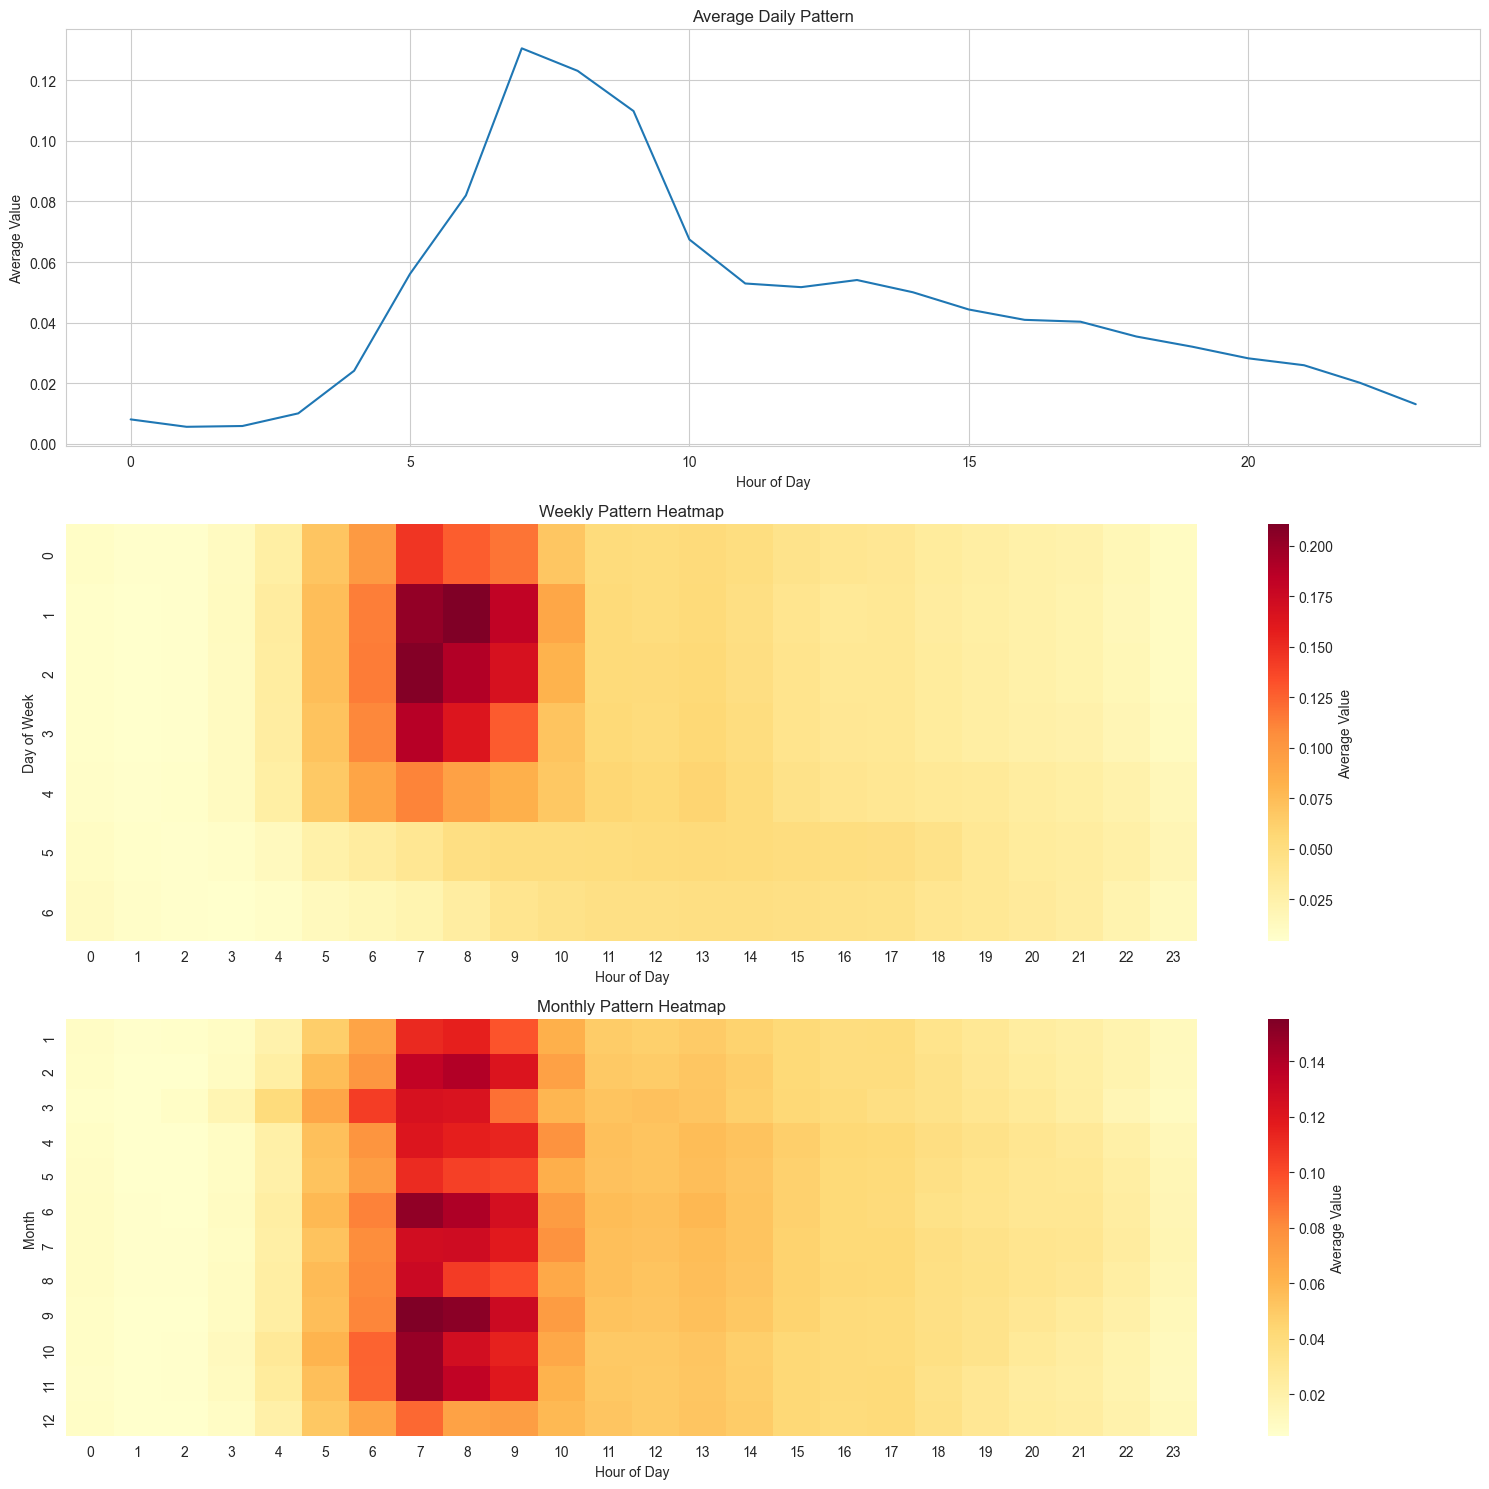
\includegraphics[width=\textwidth]{pattern_heatmaps.png}
    \caption{Pattern analysis through heatmaps: (a) Average daily pattern showing peak congestion hours, (b) Weekly pattern heatmap displaying workday vs. weekend differences, (c) Monthly pattern heatmap revealing seasonal variations.}
    \label{fig:heatmaps}
\end{figure}

To further investigate the complex temporal dynamics of traffic congestion, we employed heatmap visualizations that reveal the intricate interplay between different time scales. Figure \ref{fig:heatmaps} presents three complementary views of the temporal patterns in our data.

The daily pattern heatmap reveals a pronounced morning peak between 07:00 and 09:00, with congestion values reaching their maximum around 08:00. This peak is followed by a gradual decline throughout the day, with a subtle secondary peak during the afternoon rush hour (16:00-18:00). The lowest congestion levels are consistently observed during the early morning hours (02:00-05:00).

The weekly pattern heatmap offers a particularly insightful visualization of the workday-weekend dichotomy. Workdays (represented by rows 0-4) show consistently higher congestion levels during peak hours, with the intensity gradually diminishing towards the weekend. Rows 5 and 6, corresponding to Saturday and Sunday, display markedly lower congestion levels throughout the day, though still maintaining a vestigial morning peak structure.

The monthly pattern heatmap extends our understanding to seasonal variations throughout the year. While the basic daily pattern remains consistent across months, subtle variations in intensity can be observed. This visualization suggests that while the fundamental rhythm of traffic congestion is primarily driven by daily and weekly cycles, there are also longer-term patterns that might influence the overall congestion levels.

\begin{figure}[htbp]
    \centering
    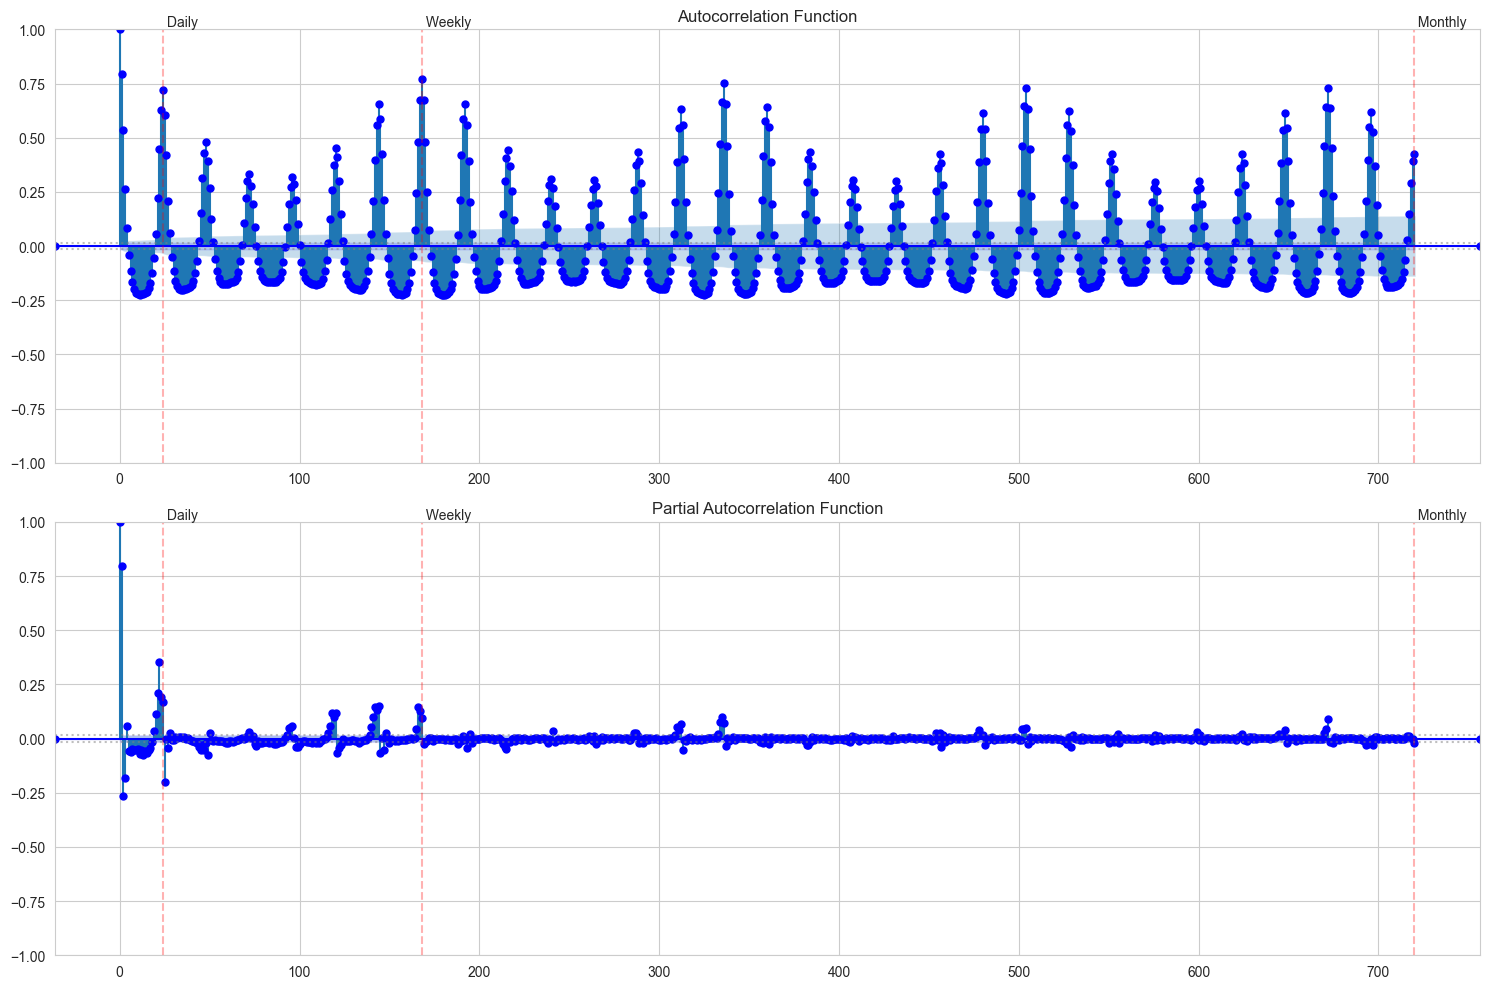
\includegraphics[width=\textwidth]{acf_pacf_extended.png}
    \caption{Extended ACF and PACF analysis showing correlations at different time scales: daily (24 hours), weekly (168 hours), and monthly (720 hours) patterns.}
    \label{fig:acf_extended}
\end{figure}

The extended correlation analysis (Figure \ref{fig:acf_extended}) provides a quantitative confirmation of these visual patterns. The ACF exhibits clear periodicity at multiple time scales:

\begin{itemize}
    \item \textbf{Daily Periodicity}: Strong correlations at 24-hour intervals, with peaks gradually diminishing but remaining significant.
    \item \textbf{Weekly Periodicity}: Secondary peaks at 168-hour (7-day) intervals, indicating the weekly cycle's persistence.
    \item \textbf{Monthly Effects}: Weaker but detectable correlations at approximately 720-hour intervals, suggesting potential monthly patterns.
\end{itemize}

The PACF analysis reveals the direct correlations at these lags after removing the effects of intermediate observations. The sharp cut-off in the PACF after the first few lags, combined with the oscillating decay in the ACF, suggests that a combination of autoregressive and moving average terms will be necessary to capture these multi-scale patterns effectively.

This rich temporal structure informs our modeling strategy in several ways:
\begin{enumerate}
    \item The need for explicit handling of both daily and weekly seasonality
    \item The importance of capturing the sharp morning peak characteristics
    \item The requirement for flexibility in modeling different intensities between workdays and weekends
    \item The potential value of incorporating longer-term variations in the model structure
\end{enumerate}

\section{Model Selection and Specification}

\subsection{ARIMA Model Family}

The selection and specification of our ARIMA model followed a systematic approach, incorporating both statistical analysis and domain knowledge of traffic patterns. Our final specification converged on a SARIMAX(2,1,2)(1,1,1)$_{24}$ model with exogenous variables capturing weekly patterns, representing a careful balance between model complexity and forecasting capability.

\subsubsection{Stationarity and Differencing Analysis}
Initial analysis of the time series revealed complex seasonal patterns at both daily and weekly frequencies. While the Augmented Dickey-Fuller test indicated statistical stationarity (test statistic -15.71, p-value 1.37×10$^{-28}$), visual inspection of the ACF and PACF plots suggested that differencing could simplify the underlying patterns:

\begin{itemize}
    \item \textbf{Regular Differencing}: First-order differencing ($d=1$) was applied to address short-term dependencies and simplify the correlation structure
    \item \textbf{Seasonal Differencing}: A seasonal difference ($D=1$) at lag 24 was incorporated to handle the pronounced daily seasonality
\end{itemize}

This differencing strategy effectively transformed the series into a more manageable form while preserving its essential characteristics.

\subsubsection{Order Selection Process}
The determination of model orders followed a rigorous analysis of the differenced series' correlation structure:

\textbf{Regular Components}:
\begin{itemize}
    \item Autoregressive order $p=2$: Selected based on significant PACF spikes at lags 1 and 2, capturing short-term traffic dependency patterns
    \item Moving average order $q=2$: Chosen to address the residual correlation structure evident in the ACF at low lags
\end{itemize}

\textbf{Seasonal Components}:
\begin{itemize}
    \item Seasonal AR order $P=1$: Determined from significant seasonal PACF spikes at lag 24
    \item Seasonal MA order $Q=1$: Indicated by the ACF pattern at seasonal lags
\end{itemize}

The resulting model can be expressed mathematically as:

\begin{equation}
(1-\phi_1B-\phi_2B^2)(1-\Phi_1B^{24})(1-B)(1-B^{24})X_t = (1+\theta_1B+\theta_2B^2)(1+\Theta_1B^{24})\varepsilon_t + \beta W_t
\end{equation}

where $B$ is the backshift operator, $\phi_i$ and $\theta_i$ are the regular AR and MA parameters, $\Phi_1$ and $\Theta_1$ are the seasonal parameters, and $W_t$ represents the exogenous weekly pattern variable.

\subsubsection{Seasonal Component Integration}
The seasonal component of our model addresses two distinct cyclic patterns:

1. \textbf{Daily Seasonality}: Explicitly modeled through the seasonal ARIMA structure with period 24, capturing the regular daily traffic cycles:
   \begin{equation}
   (1-\Phi_1B^{24})(1-B^{24})X_t
   \end{equation}

2. \textbf{Weekly Pattern}: Incorporated through an exogenous variable using a phase-adjusted sine component:
   \begin{equation}
   W_t = \sin(2\pi f_w t + \phi)
   \end{equation}
   where $f_w$ represents the weekly frequency and $\phi$ is a phase adjustment optimized to align with observed traffic patterns.

\subsubsection{Final Model Specification Rationale}
The final SARIMAX(2,1,2)(1,1,1)$_{24}$ specification was chosen based on several key considerations:

\begin{itemize}
    \item \textbf{Model Parsimony}: The selected orders provide sufficient complexity to capture relevant patterns while avoiding overfitting
    \item \textbf{Information Criteria}: AIC and BIC values supported this specification over alternatives
    \item \textbf{Residual Analysis}: The model produces well-behaved residuals with minimal remaining autocorrelation
    \item \textbf{Forecast Stability}: The specification demonstrates stable behavior in out-of-sample testing
\end{itemize}

The inclusion of the exogenous weekly pattern variable enhances the model's ability to capture regular traffic variations while maintaining interpretability. This hybrid approach, which combines traditional SARIMA components with exogenous variables, provides a robust framework for capturing both the short-term dynamics and the longer-term patterns inherent in traffic congestion data.

\subsubsection{Holiday Pattern Integration}
A key enhancement to our SARIMAX model involves the explicit handling of Christmas period traffic patterns. Analysis of historical data from 2015 revealed significant variations in traffic behavior during the Christmas period, necessitating special treatment in our modeling approach.

To quantify this effect, we conducted a detailed analysis of traffic patterns during Christmas 2015, focusing specifically on daytime hours (08:00-20:00) on December 24th and 25th. Our methodology involved:

\begin{enumerate}
    \item \textbf{Baseline Comparison}: We compared actual traffic volumes during Christmas daytime hours against model-predicted values for the same period
    \item \textbf{Ratio Calculation}: For each Christmas day, we computed the ratio:
    \begin{equation}
        r_d = \frac{\text{Actual Traffic Volume}}{\text{Model Predicted Volume}}
    \end{equation}
    where $d \in \{24, 25\}$ represents December 24th and 25th respectively
\end{enumerate}

This analysis revealed systematic differences between normal model predictions and actual Christmas traffic patterns:

\begin{itemize}
    \item December 24th showed a traffic reduction ratio of approximately 0.65
    \item December 25th exhibited an even stronger effect with a ratio of approximately 0.47
\end{itemize}

Based on these findings, we developed a Christmas dampening factor $\alpha$:
\begin{equation}
    \alpha = \frac{1}{2}\sum_{d \in \{24,25\}} r_d \approx 0.56
\end{equation}

This dampening factor was incorporated into our forecasting framework through a modification of the prediction equation during Christmas periods:
\begin{equation}
    \hat{X}_t^* = \begin{cases}
        \alpha \hat{X}_t & \text{if } t \in \text{Christmas daytime hours} \\
        \hat{X}_t & \text{otherwise}
    \end{cases}
\end{equation}

where $\hat{X}_t$ represents the standard model forecast and $\hat{X}_t^*$ represents the adjusted forecast that accounts for Christmas effects.

This approach allows our model to maintain its standard performance during regular periods while appropriately adjusting predictions during Christmas daytime hours, reflecting the historically observed reduction in traffic volumes during this special period.

\subsubsection{Model Estimation Results}

The estimation of our final SARIMAX specification demonstrates strong statistical significance across all components. Table \ref{tab:sarimax_results} presents the complete parameter estimates and model diagnostics.

\begin{table}[htbp]
    \centering
    \caption{SARIMAX Model Results}
    \label{tab:sarimax_results}
    \begin{tabular}{lrrrrc}
        \toprule
        Parameter & Coefficient & Std. Error & z-value & P$>|$z$|$ & [0.025 \quad 0.975] \\
        \midrule
        day\_sin & -0.0055 & 0.002 & -2.883 & 0.004 & [-0.009 \quad -0.002] \\
        ar.L1 & 0.3634 & 0.076 & 4.788 & 0.000 & [0.215 \quad 0.512] \\
        ar.L2 & 0.1545 & 0.058 & 2.671 & 0.008 & [0.041 \quad 0.268] \\
        ma.L1 & -0.5933 & 0.074 & -7.982 & 0.000 & [-0.739 \quad -0.448] \\
        ma.L2 & -0.3790 & 0.076 & -4.989 & 0.000 & [-0.528 \quad -0.230] \\
        ar.S.L24 & 0.3275 & 0.004 & 75.000 & 0.000 & [0.319 \quad 0.336] \\
        ma.S.L24 & -0.9899 & 0.001 & -990.119 & 0.000 & [-0.992 \quad -0.988] \\
        sigma2 & 0.0006 & 3.07×10$^{-6}$ & 196.772 & 0.000 & [0.001 \quad 0.001] \\
        \midrule
        \multicolumn{6}{l}{Model Statistics} \\
        \midrule
        Log Likelihood & 18129.444 & \multicolumn{2}{l}{Observations} & \multicolumn{2}{l}{8016} \\
        AIC & -36242.888 & \multicolumn{2}{l}{Ljung-Box (Q)} & \multicolumn{2}{l}{1.09} \\
        BIC & -36187.027 & \multicolumn{2}{l}{Prob(Q)} & \multicolumn{2}{l}{0.30} \\
        HQIC & -36223.763 & \multicolumn{2}{l}{Jarque-Bera (JB)} & \multicolumn{2}{l}{122072.30} \\
        & & \multicolumn{2}{l}{Prob(JB)} & \multicolumn{2}{l}{0.00} \\
        \bottomrule
    \end{tabular}
\end{table}

The parameter estimates reveal several key insights:
\begin{itemize}
    \item Strong statistical significance across all components (p < 0.01)
    \item Particularly robust seasonal effects, with the seasonal MA term (ma.S.L24) showing exceptionally high precision
    \item Significant weekly pattern component (day\_sin), confirming the importance of our weekly cycle adjustment
    \item Well-behaved residuals with no significant autocorrelation (Ljung-Box Q = 1.09, p = 0.30)
\end{itemize}

The high significance of both regular and seasonal components supports our model specification choices, while the favorable information criteria (AIC: -36242.888, BIC: -36187.027) suggest we have achieved a good balance between model complexity and fit.

\subsubsection{Visual Analysis and Model Output}

The development of our ARIMA model's Christmas adjustment was motivated by careful analysis of historical patterns. Figure \ref{fig:christmas_2015} presents the traffic congestion patterns observed during November-December 2015, with the Christmas period highlighted in red.

\begin{figure}[htbp]
    \centering
    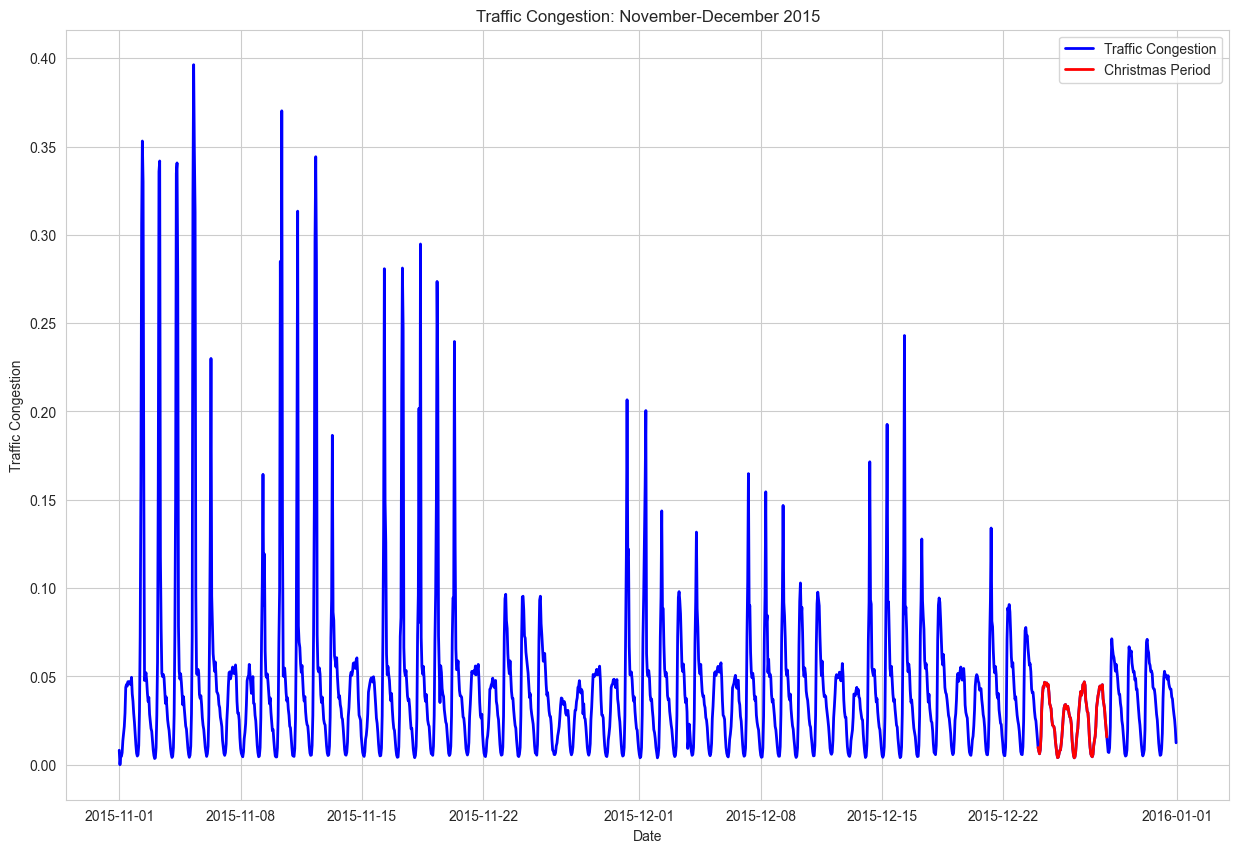
\includegraphics[width=\textwidth]{christmas_2015.png}
    \caption{Traffic congestion patterns for November-December 2015. The red segment highlights the Christmas period, showing notably reduced congestion levels compared to regular patterns.}
    \label{fig:christmas_2015}
\end{figure}

This visualization shows a possible behavior during the Christmas period, characterized by substantially reduced congestion levels compared to typical patterns. Of particular note is the systematic reduction in peak congestion values during the highlighted period, supporting our quantitative finding of a dampening factor $\alpha \approx 0.56$ during daytime hours.

The application of our final SARIMAX model, incorporating both the seasonal components and the Christmas dampening effect, is illustrated in Figure \ref{fig:arima_forecast}.

\begin{figure}[htbp]
    \centering
    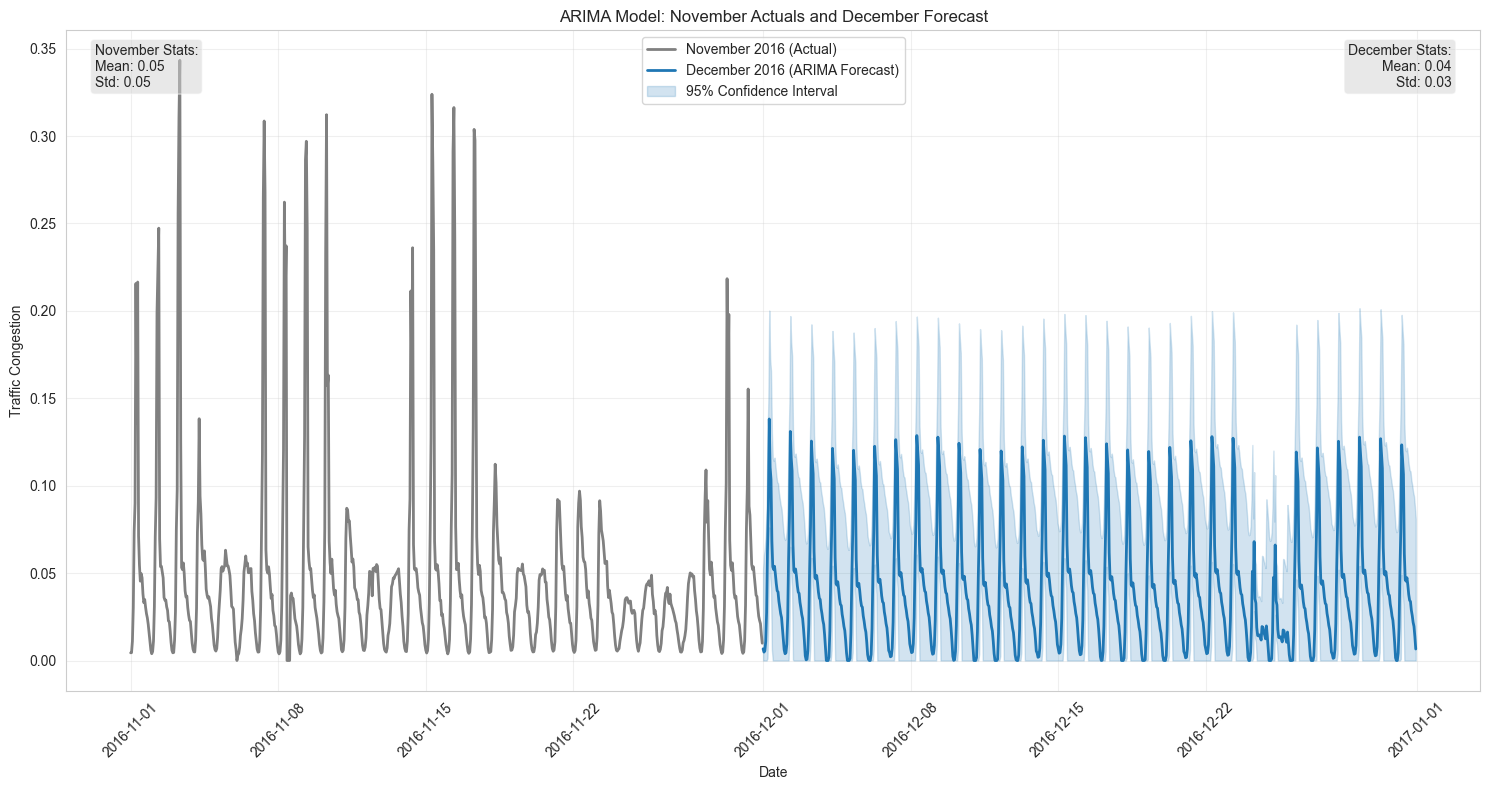
\includegraphics[width=\textwidth]{arima_forecast.png}
    \caption{ARIMA model forecast with November 2016 historical data (gray) and December forecast (blue) including 95\% confidence intervals (light blue shading). The forecast exhibits both the underlying seasonal pattern and the Christmas period adjustment.}
    \label{fig:arima_forecast}
\end{figure}

The forecast visualization demonstrates several key features of our modeling approach:

\begin{itemize}
    \item \textbf{Seasonal Continuity}: The forecasted values (blue line) maintain the daily and weekly seasonal patterns observed in the November data (gray line)
    
    \item \textbf{Christmas Adjustment}: The forecast shows a visible dampening effect during the Christmas period, reflecting our historically-informed adjustment
    
    \item \textbf{Uncertainty Quantification}: The 95\% confidence intervals (light blue shading) provide a measure of forecast uncertainty, appropriately widening as the forecast extends further into the future
    
    \item \textbf{Pattern Stability}: The mean and standard deviation statistics shown in the plot corners indicate that the forecast maintains reasonable statistical properties compared to the historical data
\end{itemize}

The confidence intervals deserve particular attention, as they capture both the inherent variability in traffic patterns and the additional uncertainty introduced by holiday effects. The widening of these intervals during the Christmas period reflects the increased forecasting complexity during this unusual period.

\subsection{Unobserved Components Model (UCM)}

Our second modeling approach employs an Unobserved Components Model framework, which decomposes the traffic congestion time series into interpretable components while incorporating exogenous variables for enhanced accuracy. This approach provides flexibility in capturing evolving patterns while maintaining interpretability of the individual components.

\subsubsection{Component Structure Analysis}
The UCM framework decomposes the traffic congestion series $X_t$ into several components:

\begin{equation}
X_t = \mu_t + \sum_{h=5}^{14} \beta_h D_{h,t} + \varepsilon_t
\end{equation}

where:
\begin{itemize}
    \item $\mu_t$ represents the local level component
    \item $D_{h,t}$ are dummy variables for significant hours (5:00-14:00)
    \item $\beta_h$ are the corresponding coefficients for each hour
    \item $\varepsilon_t$ is the irregular component
\end{itemize}

\textbf{Level Component Design:}
The local level component $\mu_t$ follows a random walk process:
\begin{equation}
\mu_t = \mu_{t-1} + \eta_t, \quad \eta_t \sim N(0, \sigma^2_\eta)
\end{equation}

This specification allows the underlying level to evolve smoothly over time, capturing gradual changes in baseline traffic congestion while maintaining stability in the short term.

\textbf{Hour-Specific Effects:}
Analysis of traffic patterns revealed that certain hours consistently demonstrate distinct behavior. Rather than implementing a full 24-hour seasonal component, our refined approach focuses on the most significant hours (5:00-14:00), capturing the morning rush period and subsequent transition. This selective approach reduces model complexity while maintaining predictive power.

\subsubsection{Parameter Specification Process}
The parameter estimation process followed a systematic approach:

1. \textbf{Variance Components:}
   \begin{itemize}
       \item Level variance $\sigma^2_\eta$: Estimated to balance between stability and adaptivity
       \item Irregular variance $\sigma^2_\varepsilon$: Captures short-term fluctuations
   \end{itemize}

2. \textbf{Hour Coefficients:}
   \begin{itemize}
       \item $\beta_h$ parameters estimated via maximum likelihood
       \item Significance tests guided the selection of relevant hours
   \end{itemize}

3. \textbf{Initial State:}
   \begin{itemize}
       \item Initial level $\mu_0$ determined from early observations
       \item Diffuse prior used for initialization uncertainty
   \end{itemize}

\subsubsection{Model Structure Justification}
The refined UCM specification was chosen based on several key considerations:

\begin{itemize}
    \item \textbf{Parsimony}: Focus on significant hours reduces parameter count while maintaining explanatory power
    \item \textbf{Interpretability}: Each component has a clear physical meaning in terms of traffic patterns
    \item \textbf{Flexibility}: Local level component adapts to gradual changes in traffic patterns
    \item \textbf{Hour-Specific Effects}: Explicit modeling of peak hours captures crucial daily variation
\end{itemize}

The model estimation revealed that hours 5 through 14 exhibit the strongest systematic effects, aligning with intuitive understanding of morning traffic patterns. The significance of these hours was determined through a combination of likelihood ratio tests and analysis of coefficient stability.

\subsubsection{Holiday Period Treatment}
Following the insights gained from the ARIMA analysis, our UCM implementation also incorporates special treatment for the Christmas period. This is achieved through a modification of the observation equation during holiday periods:

\begin{equation}
X_t = \begin{cases}
    \alpha(\mu_t + \sum_{h=5}^{14} \beta_h D_{h,t}) + \varepsilon_t & \text{if } t \in \text{Christmas daytime} \\
    \mu_t + \sum_{h=5}^{14} \beta_h D_{h,t} + \varepsilon_t & \text{otherwise}
\end{cases}
\end{equation}

where $\alpha$ is the dampening factor derived from historical holiday pattern analysis.

This structure maintains the model's core ability to capture regular patterns while appropriately adjusting predictions during known anomalous periods. The combination of hour-specific effects and holiday adjustment provides a robust framework for capturing both regular and exceptional traffic patterns.

\subsubsection{Model Estimation and Visual Analysis}

The estimation results of our refined UCM specification reveal strong statistical support for the selected model structure. Table \ref{tab:ucm_results} presents the complete parameter estimates and their statistical significance.

\begin{table}[htbp]
    \centering
    \caption{Unobserved Components Model Results}
    \label{tab:ucm_results}
    \begin{tabular}{lrrrrc}
        \toprule
        Parameter & Coefficient & Std. Error & z-value & P$>|$z$|$ & [0.025 \quad 0.975] \\
        \midrule
        $\sigma^2_{\text{irregular}}$ & 1.091×10$^{-5}$ & 2.5×10$^{-6}$ & 4.356 & 0.000 & [6.00×10$^{-6}$ \quad 1.58×10$^{-5}$] \\
        $\sigma^2_{\text{level}}$ & 0.0007 & 6.66×10$^{-6}$ & 103.983 & 0.000 & [0.001 \quad 0.001] \\
        $\beta_{\text{hour\_5}}$ & 0.0303 & 0.002 & 19.521 & 0.000 & [0.027 \quad 0.033] \\
        $\beta_{\text{hour\_6}}$ & 0.0543 & 0.002 & 30.710 & 0.000 & [0.051 \quad 0.058] \\
        $\beta_{\text{hour\_7}}$ & 0.1010 & 0.002 & 55.122 & 0.000 & [0.097 \quad 0.105] \\
        $\beta_{\text{hour\_8}}$ & 0.0917 & 0.002 & 47.812 & 0.000 & [0.088 \quad 0.095] \\
        $\beta_{\text{hour\_9}}$ & 0.0766 & 0.002 & 38.602 & 0.000 & [0.073 \quad 0.080] \\
        $\beta_{\text{hour\_10}}$ & 0.0323 & 0.002 & 16.066 & 0.000 & [0.028 \quad 0.036] \\
        $\beta_{\text{hour\_11}}$ & 0.0159 & 0.002 & 7.402 & 0.000 & [0.012 \quad 0.020] \\
        $\beta_{\text{hour\_12}}$ & 0.0129 & 0.005 & 2.658 & 0.008 & [0.003 \quad 0.022] \\
        $\beta_{\text{hour\_13}}$ & 0.0134 & 0.005 & 2.736 & 0.006 & [0.004 \quad 0.023] \\
        $\beta_{\text{hour\_14}}$ & 0.0076 & 0.004 & 1.790 & 0.073 & [-0.001 \quad 0.016] \\
        \midrule
        \multicolumn{6}{l}{Model Statistics} \\
        \midrule
        Log Likelihood & 37004.331 & \multicolumn{2}{l}{Observations} & \multicolumn{2}{l}{16800} \\
        AIC & -73984.663 & \multicolumn{2}{l}{Ljung-Box (Q)} & \multicolumn{2}{l}{0.04} \\
        BIC & -73891.914 & \multicolumn{2}{l}{Prob(Q)} & \multicolumn{2}{l}{0.84} \\
        HQIC & -73954.060 & \multicolumn{2}{l}{Heteroskedasticity (H)} & \multicolumn{2}{l}{0.93} \\
        & & \multicolumn{2}{l}{Prob(H)} & \multicolumn{2}{l}{0.01} \\
        \bottomrule
    \end{tabular}
\end{table}

The parameter estimates reveal several key insights:
\begin{itemize}
    \item A clear progression in the hour coefficients, with the strongest effects during the morning rush period (hours 7-9)
    \item Well-identified variance components for both irregular and level terms
    \item Declining significance of hour effects into the afternoon, with hour 14 being marginally significant
    \item Strong overall model fit, evidenced by the high log-likelihood and favorable information criteria
\end{itemize}

Figure \ref{fig:ucm_forecast} presents the model's forecast alongside historical November data.

\begin{figure}[htbp]
    \centering
    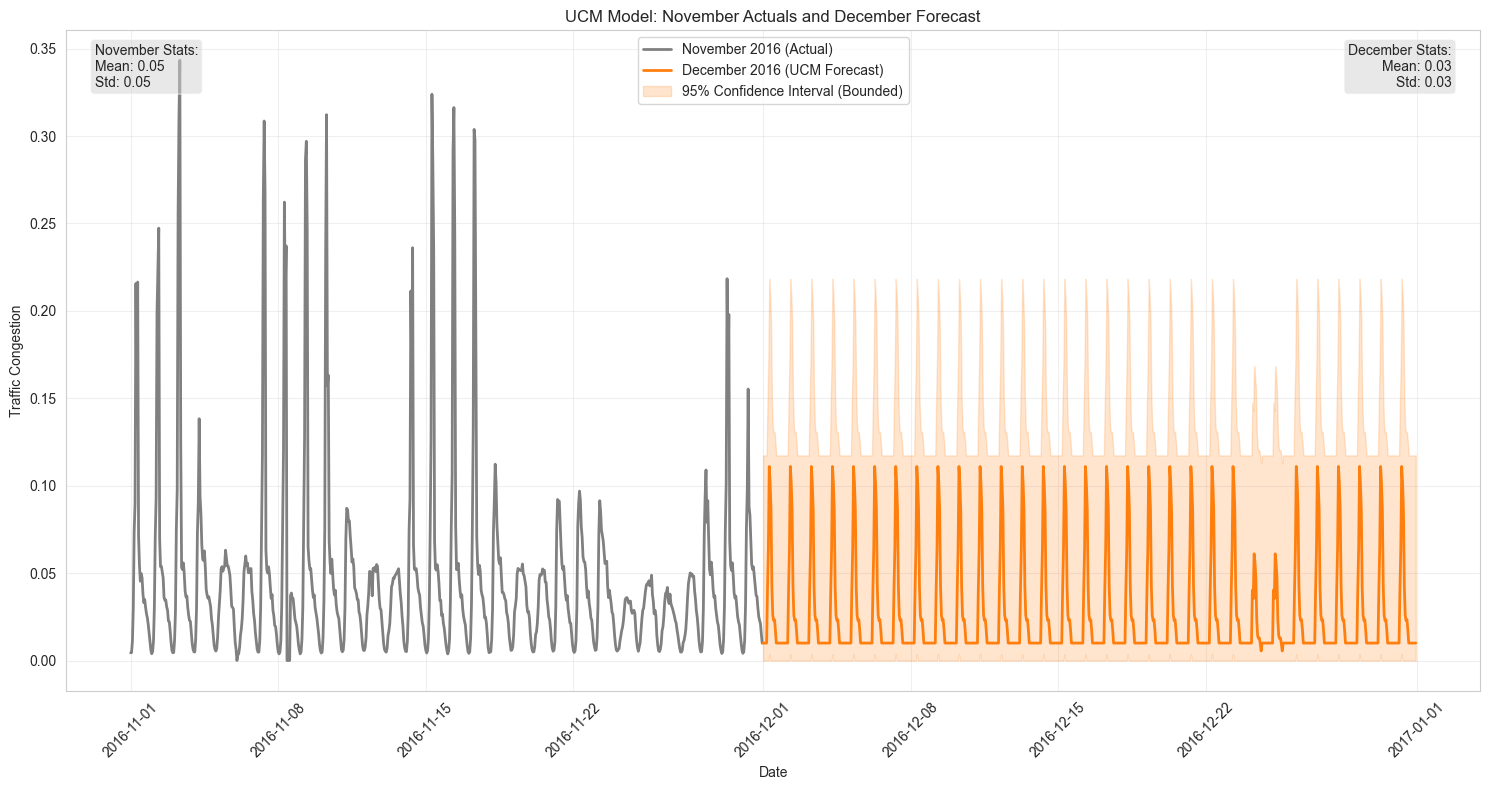
\includegraphics[width=\textwidth]{ucm_forecast.png}
    \caption{UCM model forecast with November 2016 historical data (gray) and December forecast (orange) including bounded 95\% confidence intervals (light orange shading). The forecast exhibits both the hour-specific effects and the Christmas period adjustment.}
    \label{fig:ucm_forecast}
\end{figure}

The forecast visualization demonstrates several notable features:

\begin{itemize}
    \item \textbf{Hour-Specific Patterns}: The morning peak effects are clearly visible, with the strongest impacts during hours 7-9 ($\beta_{hour\_7} = 0.1010$, $\beta_{hour\_8} = 0.0917$, $\beta_{hour\_9} = 0.0766$)
    
    \item \textbf{Level Stability}: The local level component ($\sigma^2_{level} = 0.0007$) provides a stable baseline while allowing for gradual adjustments
    
    \item \textbf{Bounded Uncertainty}: The confidence intervals are constrained based on historical volatility patterns, providing more realistic uncertainty quantification
    
    \item \textbf{Holiday Adjustment}: The Christmas period shows appropriate dampening of the hour-specific effects
\end{itemize}

The model's statistical diagnostics are strong, with no significant residual autocorrelation (Ljung-Box Q = 0.04, p = 0.84). Some heteroskedasticity is present (H = 0.93, p = 0.01), which is addressed through our bounded confidence interval approach. This combination of flexible modeling and empirically-grounded uncertainty quantification provides a robust framework for capturing the complex patterns in traffic congestion.



\end{document}
